\documentclass[hyperref, a4paper]{article}

\usepackage{geometry}
\usepackage{titling}
\usepackage{titlesec}
% No longer needed, since we will use enumitem package
% \usepackage{paralist}
\usepackage{enumitem}
\usepackage{footnote}
\usepackage{enumerate}
\usepackage{amsmath, amssymb, amsthm}
\usepackage{mathtools}
\usepackage{bbm}
\usepackage{cite}
\usepackage{graphicx}
\usepackage{subfigure}
\usepackage{physics}
\usepackage{tensor}
\usepackage{siunitx}
\usepackage[version=4]{mhchem}
\usepackage{tikz}
\usepackage{xcolor}
\usepackage{listings}
\usepackage{autobreak}
\usepackage[ruled, vlined, linesnumbered]{algorithm2e}
\usepackage{nameref,zref-xr}
\zxrsetup{toltxlabel}
\usepackage[colorlinks,unicode]{hyperref} % , linkcolor=black, anchorcolor=black, citecolor=black, urlcolor=black, filecolor=black
\usepackage[most]{tcolorbox}
\usepackage{prettyref}

% Page style
\geometry{left=3.18cm,right=3.18cm,top=2.54cm,bottom=2.54cm}
\titlespacing{\paragraph}{0pt}{1pt}{10pt}[20pt]
\setlength{\droptitle}{-5em}

% More compact lists 
\setlist[itemize]{
    itemindent=17pt, 
    leftmargin=1pt,
    listparindent=\parindent,
    parsep=0pt,
}

% Math operators
\DeclareMathOperator{\timeorder}{\mathcal{T}}
\DeclareMathOperator{\diag}{diag}
\DeclareMathOperator{\legpoly}{P}
\DeclareMathOperator{\primevalue}{P}
\DeclareMathOperator{\sgn}{sgn}
\DeclareMathOperator{\res}{Res}
\newcommand*{\ii}{\mathrm{i}}
\newcommand*{\ee}{\mathrm{e}}
\newcommand*{\const}{\mathrm{const}}
\newcommand*{\suchthat}{\quad \text{s.t.} \quad}
\newcommand*{\argmin}{\arg\min}
\newcommand*{\argmax}{\arg\max}
\newcommand*{\normalorder}[1]{: #1 :}
\newcommand*{\pair}[1]{\langle #1 \rangle}
\newcommand*{\fd}[1]{\mathcal{D} #1}
\DeclareMathOperator{\bigO}{\mathcal{O}}

% TikZ setting
\usetikzlibrary{arrows,shapes,positioning}
\usetikzlibrary{arrows.meta}
\usetikzlibrary{decorations.markings}
\tikzstyle arrowstyle=[scale=1]
\tikzstyle directed=[postaction={decorate,decoration={markings,
    mark=at position .5 with {\arrow[arrowstyle]{stealth}}}}]
\tikzstyle ray=[directed, thick]
\tikzstyle dot=[anchor=base,fill,circle,inner sep=1pt]

% Algorithm setting
% Julia-style code
\SetKwIF{If}{ElseIf}{Else}{if}{}{elseif}{else}{end}
\SetKwFor{For}{for}{}{end}
\SetKwFor{While}{while}{}{end}
\SetKwProg{Function}{function}{}{end}
\SetArgSty{textnormal}

\newcommand*{\concept}[1]{{\textbf{#1}}}

% Embedded codes
\lstset{basicstyle=\ttfamily,
  showstringspaces=false,
  commentstyle=\color{gray},
  keywordstyle=\color{blue}
}

% Reference formatting
\newrefformat{fig}{Figure~\ref{#1}}

% Color boxes
\tcbuselibrary{skins, breakable, theorems}
\newtcbtheorem[number within=section]{warning}{Warning}%
  {colback=orange!5,colframe=orange!65,fonttitle=\bfseries, breakable}{warn}
\newtcbtheorem[number within=section]{note}{Note}%
  {colback=green!5,colframe=green!65,fonttitle=\bfseries, breakable}{note}
\newtcbtheorem[number within=section]{info}{Info}%
  {colback=blue!5,colframe=blue!65,fonttitle=\bfseries, breakable}{info}

\newenvironment{shelldisplay}{\begin{lstlisting}}{\end{lstlisting}}

\title{Homework 3}
\author{Jinyuan Wu}

\begin{document}

\maketitle

\paragraph{Lecture 8, Exercise 3}

\paragraph{Solution} We have 
\[
    U = I_1 R = \frac{1}{C} \int \dd{t} I_2 = L \dv{I_3}{t},
\]
and 
\[
    I = I_1 + I_2 + I_3.
\]
In the frequency domain, we have 
\[
    U[\omega] = I_1[\omega] R = \frac{1}{C} \frac{1}{- \ii \omega} I_2 = L (- \ii \omega) I_3,
\]
and therefore 
\begin{equation}
    Z[\omega] = \frac{U[\omega]}{I_1[\omega] + I_2[\omega] + I_3[\omega]} 
    = \frac{1}{\frac{1}{R} - \ii \omega C - \frac{1}{\ii \omega L}}.
\end{equation}
So we have 
\begin{equation}
    \Re Z[\omega] = \frac{1}{R} \frac{1}{\frac{1}{R^2} + \left( \frac{1}{\omega L} - \omega C \right)^2},
\end{equation}
and 
\begin{equation}
    \Im Z[\omega] = - \left( \frac{1}{\omega L} - \omega C \right) \frac{1}{\frac{1}{R^2} + \left( \frac{1}{\omega L} - \omega C \right)^2}.
\end{equation}
The zero points of the denominator are given by 
\begin{equation}
    \omega = \omega_{1, 2} \coloneqq \frac{- \frac{\ii}{R} \pm \sqrt{- \frac{1}{R^2} + \frac{4C}{L}}}{2 C}.
\end{equation}
It can be easily verified that the zero points of 
\[
    \frac{1}{R^2} + \left( \frac{1}{\omega L} - \omega C \right)^2
\]
are $\omega_{1, 2}$ and $\omega_{1, 2}^*$.
So we have 
\begin{equation}
    \Re Z[\omega] = \frac{1}{R} \frac{\omega^2}{C^2 
    (\omega - \omega_1) (\omega - \omega_2) (\omega - \omega_1^*) (\omega - \omega_2^*)},
\end{equation}
and 
\begin{equation}
    \Im Z[\omega] = - \left(\frac{\omega}{L} - \omega^3 C \right) 
    \frac{1}{C^2 
    (\omega - \omega_1) (\omega - \omega_2) (\omega - \omega_1^*) (\omega - \omega_2^*)}.
\end{equation}
So now let's show that 
\begin{equation}
    \Im Z[\omega] = \frac{1}{\pi} \mathrm{P} \int_{-\infty}^\infty \dd{\omega'}
    \frac{\Re Z[\omega']}{\omega - \omega'}.
    \label{eq:k-k-1}
\end{equation}
Since both $\Re Z[\omega]$ and $\Im Z[\omega]$ are well-behaved at $\omega \to \infty$,
we can just apply the residue theorem to the upper plane or the lower plane -- 
here we choose the upper plane, and 
\[
    \begin{aligned}
        \mathrm{P} \int_{-\infty}^\infty \dd{\omega'}
        \frac{\Re Z[\omega']}{\omega - \omega'} &= 
        - (\pi \ii \res_{\omega' = \omega} 
        + 2\pi \ii \res_{\omega' = \omega_1^*} 
        + 2\pi \ii \res_{\omega' = \omega_2^*}) \Re \frac{Z[\omega']}{\omega' - \omega} \\
        &= - \pi \ii \frac{1}{R} \frac{\omega^2}{
            C^2 (\omega - \omega_1) (\omega - \omega_2) (\omega - \omega_1^*) (\omega - \omega_2^*)
        } \\
        &\quad - 2 \pi \ii \frac{1}{\omega_1^* - \omega} \frac{1}{R} \frac{(\omega_1^*)^2}{
            C^2 (\omega_1^* - \omega_1) (\omega_1^* - \omega_2) (\omega_1^* - \omega_2^*)
        } \\
        &\quad - 2 \pi \ii \frac{1}{\omega_2^* - \omega} \frac{1}{R} \frac{(\omega_2^*)^2}{
            C^2 (\omega_2^* - \omega_1) (\omega_2^* - \omega_2) (\omega_2^* - \omega_1^*)
        }.
    \end{aligned}
\]
Comparing this equation and \eqref{eq:k-k-1}, what we need to prove is 
\begin{equation}
    \frac{2\ii}{R} \left(
        \frac{(\omega - \omega_2^*) (\omega - \omega_1) (\omega - \omega_2) (\omega_1^*)^2}{
            (\omega_1^* - \omega_1) (\omega_1^* - \omega_2) (\omega_1^* - \omega_2^*)
        } + 
        \frac{(\omega - \omega_1) (\omega - \omega_2) (\omega - \omega_1^*) (\omega_2^*)^2}{
            (\omega_2^* - \omega_1) (\omega_2^* - \omega_2) (\omega_2^* - \omega_1^*)
        }
    \right) - \ii \frac{\omega^2}{R} = - \left(\frac{\omega}{L} - \omega^3 C \right) .
\end{equation}
This can be verified by Mathematica (\prettyref{fig:notebook}).
The exact same procedure can also be used to prove 
\begin{equation}
    \Re Z[\omega] = \frac{1}{\pi} \mathrm{P} \int_{-\infty}^\infty \dd{\omega'}
    \frac{\Im Z[\omega']}{\omega' - \omega}.
    \label{eq:k-k-2}
\end{equation}

\begin{figure}
    \centering
    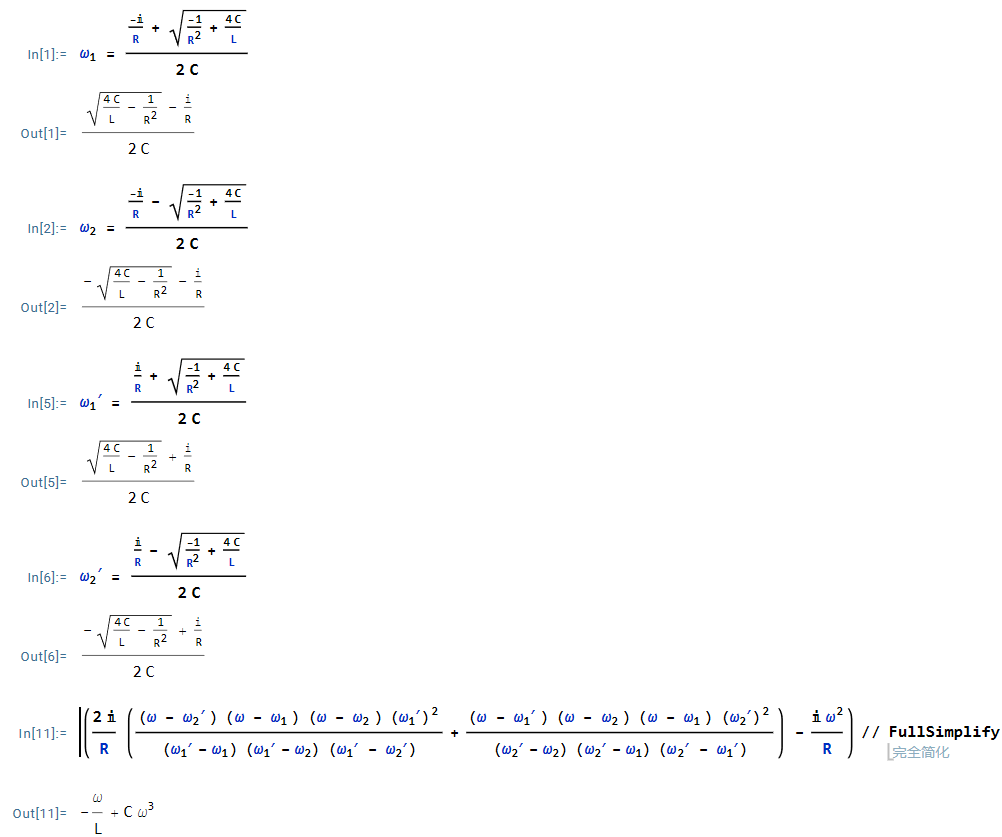
\includegraphics[width=0.7\textwidth]{software/kk-relation-1.PNG}
    \caption{A Mathematica notebook verifying \eqref{eq:k-k-1} in the underdamped case}
    \label{fig:notebook}
\end{figure}

\paragraph{Lecture 9, Exercise 3} 

\paragraph{Solution} The energy density is (see \eqref{eq:transmission-u-i-ham})
\begin{equation}
    \mathcal{E} = \frac{1}{2} c V^2 + \frac{1}{2} l I^2.
\end{equation}
Therefore since 
\begin{equation}
    \pdv{V}{x} = - l \pdv{I}{t}, \quad 
    \pdv{I}{x} = - c \pdv{V}{t},
\end{equation}
we have
\[
    \begin{aligned}
        \pdv{J}{x} &= - \pdv{\mathcal{E}}{t} = - c V \pdv{V}{t} - l I \pdv{I}{t} \\
        &= V \pdv{I}{x} + I \pdv{V}{x} = \pdv{x} (VI),
    \end{aligned}
\]
and $J$ is therefore 
($J$ can't be uniquely decided purely from the continuity equation,
but we know $V \sim E$, $I \sim \Phi \sim B$, 
and in electrodynamics we already know $J \sim E \times B$,
so the expression here agrees with the general definition)
\begin{equation}
    J = VI = \sqrt{Z} (A^{\rightarrow} + A^{\leftarrow}) \frac{1}{\sqrt{Z}} (A^{\rightarrow} - A^{\leftarrow})
    = (A^{\rightarrow})^2 - (A^{\leftarrow})^2.
\end{equation}
Since both $A^{\rightarrow}$ and $A^{\leftarrow}$ are in harmonic oscillation,
we have 
\begin{equation}
    \abs{\bar{J}} = \frac{1}{2} \abs{ \abs{A^{\rightarrow}}^2 - \abs{A^{\leftarrow}}^2 }.
\end{equation}

\paragraph{Lecture 10, Exercise 1}

\begin{equation}
    x_j(t)=a_j \sin \left(\omega_j \tau+\phi_j\right)+\int_{-\infty}^t d \tau \cos \left(\omega_j(t-\tau)\right) \dot{X}(\tau)+X(t),
    \label{eq:oscillator-eom}
\end{equation}
and
\begin{equation}
    \dot{P}=-\frac{\partial}{\partial X} V(X)+\int_{-\infty}^t d \tau K(t-\tau) \dot{X}(\tau)+\xi(t),
\end{equation}
where 
\begin{equation}
    \begin{aligned}
        K(t) &=\sum_{j=1}^M k_j \cos \left(\omega_j t\right), \\
        \xi(t) &=\sum_{j=1}^M k_j a_j \sin \left(\omega_j t+\phi_j\right).
    \end{aligned}
\end{equation}

\paragraph{Solution} In equilibrium, we have 
\begin{equation}
    a_j^2 \sim \frac{k_{\text{B}} T}{m_j \omega_j^2},
\end{equation}
and we need to compare the first two terms on RHS of \eqref{eq:oscillator-eom}.
Since we are in the equilibrium, 
the energy flowing into the particle is equal to the energy flowing out of the particle, and therefore 
\[
    \int_{-\infty}^t \dd{\tau} K(t - \tau) \dot{X} \sim \xi (t), 
\]
and therefore 
\[
    \int_{-\infty}^t d \tau \cos \left(\omega_j(t-\tau)\right) \dot{X}(\tau) \sim 
    \frac{K_{\text{single oscillator}}}{K} \xi,
\]
and 
\[
    \abs{\int_{-\infty}^t d \tau \cos \left(\omega_j(t-\tau)\right) \dot{X}(\tau)}^2 \sim 
    \frac{K_{\text{single oscillator}}^2}{K^2} k_{\text{B}} T K ,
\]
and therefore 
\[
    \frac{1}{a^2}  \abs{\int_{-\infty}^t d \tau \cos \left(\omega_j(t-\tau)\right) \dot{X}(\tau)}^2 \sim
    \frac{K_{\text{single oscillator}}^2}{K^2} \frac{K}{m \omega_j^2}
    \sim \frac{K_{\text{single oscillator}}}{K} \ll 1,
\]
and therefore the influence of $X$'s dynamics is small.

\paragraph{Lecture 11, Exercise 2}

\paragraph{Solution} The PDE problem in question is the follows:
For the bulk equations,
\begin{equation}
    \begin{aligned}
        &\pdv{A^\rightarrow}{x} + \frac{1}{v_{\text{p}}} \pdv{A^\rightarrow}{t} = 0, \quad 
         \pdv{A^\leftarrow}{x}  - \frac{1}{v_{\text{p}}} \pdv{A^\leftarrow}{t} = 0, \\
        &A^{\rightarrow} = \frac{V}{2 \sqrt{Z}} + \frac{\sqrt{Z}}{2} I, \quad 
         A^{\leftarrow } = \frac{V}{2 \sqrt{Z}} - \frac{\sqrt{Z}}{2} I.
    \end{aligned}
\end{equation}
The boundary conditions are 
\begin{equation}
    A^{\rightarrow}(d, t) = - A^{\leftarrow}(d, t), \quad 
    I(0, t) = \Theta(t) I_0.
\end{equation}
The input current is given by a current source,
so we don't need to analyze the complicated detail about how the current goes back -- 
all we need to know is somehow $I(0, t)$ is in the given form, regardless of how this is possible.
By time domain Fourier transformation, we get 
\begin{equation}
    \pdv{A^\rightarrow}{x} - \frac{\ii \omega}{v_{\text{p}}} A^{\rightarrow} = 0, \quad 
    \pdv{A^\leftarrow }{x} + \frac{\ii \omega}{v_{\text{p}}} A^{\leftarrow } = 0,
\end{equation}
and therefore 
\[
    A^{\rightarrow}[d, \omega] = \ee^{\frac{\ii \omega d}{v_{\text{p}}}} A^{\rightarrow}[0, \omega],
\]
and 
\[
    A^{\leftarrow}[d, \omega] = \ee^{- \frac{\ii \omega d}{v_{\text{p}}}} A^{\leftarrow}[0, \omega],
\]
and by the boundary condition we find 
\begin{equation}
    A^{\leftarrow}[0, \omega] = - \ee^{\frac{\ii 2 \omega d}{v_{\text{p}}}} A^{\rightarrow}[0, \omega].
\end{equation}
Its time domain version is 
\begin{equation}
    A^{\leftarrow}(0, t) = - A^{\rightarrow}\left(0, t - \frac{2 \omega d}{v_{\text{p}}}\right).
\end{equation}
In principle, we have 
\begin{equation}
    \frac{V[0, \omega]}{I[0, \omega]} = Z \frac{A^{\rightarrow} + A^{\leftarrow}}{A^{\rightarrow} - A^{\leftarrow}}
    = Z \frac{1 - \ee^{\ii 2 \omega d / v_{\text{p}}}}{1 + \ee^{\ii 2 \omega d / v_{\text{p}}}}
    = - \ii Z \tan(\frac{\omega d}{v_{\text{p}}}),
\end{equation}
and by Fourier transformation
\begin{equation}
    I[0, \omega] = \int^{\infty}_{-\infty} \ee^{\ii \omega t} \dd{t} \Theta(t) I_0 = I_0 \frac{\ii}{\omega + \ii 0^+},
\end{equation}
and therefore 
\begin{equation}
    \begin{aligned}
        V(0, t) &= \int \frac{\dd{\omega}}{2\pi} \ee^{- \ii \omega t} V[0, \omega] = 
        ZI_0 \int \frac{\dd{\omega}}{2\pi} \ee^{- \ii \omega t} 
        \tan\left(\frac{\omega d}{v_{\text{p}}}\right) \frac{1}{\omega + \ii 0^+}. 
    \end{aligned}
\end{equation}
But this method has convergence problem which I don't know how to solve.
For this specific case, it's possible to solve the problem in the time domain.
During the $t < 0$ period, $A^{\leftarrow, \rightarrow}$, $U$ and $I$ are all zero,
so in the $0 < t < 2 \omega d / v_{\text{p}}$ period, 
$A^{\leftarrow}(0, t)$ is zero,
and therefore 
\begin{equation}
    V(0, t) = \sqrt{Z} (A^{\leftarrow}(0, t) + A^{\rightarrow}(0, t)) 
    = 2 \cdot \sqrt{Z} \cdot \frac{\sqrt{Z}}{2} \cdot I_0 \Theta(t) = Z I_0.
\end{equation}
When $2 \omega d / v_{\text{p}} < t < 4 \omega d / v_{\text{p}}$, however, we have 
\begin{equation}
    \begin{aligned}
        A^{\leftarrow}(0, t) &= - A^{\rightarrow}\left(0, t - \frac{2 \omega d}{v_{\text{p}}}\right)
        = - \frac{V\left(0, t - \frac{2 \omega d}{v_{\text{p}}}\right)}{2 \sqrt{Z}} - 
        \frac{\sqrt{Z}}{2} I\left(0, t - \frac{2 \omega d}{v_{\text{p}}}\right) \\
        &= - \sqrt{Z} I_0,
    \end{aligned}
\end{equation}
and therefore 
\begin{equation}
    V(0, t) = \sqrt{Z} (A^{\leftarrow}(0, t) + A^{\rightarrow}(0, t)) = 0.
\end{equation}
Repeating this procedure, we get 
\begin{equation}
    V(0, t) = \begin{cases}
        Z I_0, &\quad 2n \frac{2 \omega d}{v_{\text{p}}} < t < (2n+1) \frac{2 \omega d}{v_{\text{p}}}, \\
        0    , &\quad (2n+1) \frac{2 \omega d}{v_{\text{p}}} < t < (2n+2) \frac{2 \omega d}{v_{\text{p}}},
    \end{cases} \quad 
    n = 0, 1, 2, \ldots
\end{equation}

\paragraph{Problem} 

\begin{figure}
    \centering
    \begin{tikzpicture}[x=0.75pt,y=0.75pt,yscale=-1,xscale=1]
    %uncomment if require: \path (0,300); %set diagram left start at 0, and has height of 300
    
    %Shape: Arc [id:dp5331133978803468] 
    \draw  [draw opacity=0] (179.13,164.25) .. controls (175.44,163.61) and (172.51,155.1) .. (172.51,144.7) .. controls (172.51,134.08) and (175.56,125.44) .. (179.36,125.12) -- (179.58,144.7) -- cycle ; \draw  [color={rgb, 255:red, 155; green, 155; blue, 155 }  ,draw opacity=1 ] (179.13,164.25) .. controls (175.44,163.61) and (172.51,155.1) .. (172.51,144.7) .. controls (172.51,134.08) and (175.56,125.44) .. (179.36,125.12) ;  
    %Straight Lines [id:da12247143299984486] 
    \draw    (300.46,109.33) -- (319.83,109.33) ;
    %Straight Lines [id:da6109342480428939] 
    \draw    (319.83,109.33) -- (389.83,109.33) ;
    %Shape: Capacitor [id:dp8125842692023104] 
    \draw   (319.83,109.33) -- (319.83,143.9) (332.58,151.58) -- (307.08,151.58) (332.58,143.9) -- (307.08,143.9) (319.83,151.58) -- (319.83,186.15) ;
    %Shape: Capacitor [id:dp3820330659104405] 
    \draw   (389.83,109.33) -- (389.83,143.9) (402.58,151.58) -- (377.08,151.58) (402.58,143.9) -- (377.08,143.9) (389.83,151.58) -- (389.83,186.15) ;
    %Shape: Inductor (Air Core) [id:dp21252438201509394] 
    \draw   (389.83,186.15) -- (377.23,186.15) .. controls (377.23,191.11) and (374.72,195.15) .. (371.63,195.15) .. controls (368.54,195.15) and (366.03,191.11) .. (366.03,186.15) .. controls (366.03,191.11) and (363.52,195.15) .. (360.43,195.15) .. controls (357.34,195.15) and (354.83,191.11) .. (354.83,186.15) .. controls (354.83,191.11) and (352.32,195.15) .. (349.23,195.15) .. controls (346.14,195.15) and (343.63,191.11) .. (343.63,186.15) .. controls (343.63,191.11) and (341.12,195.15) .. (338.03,195.15) .. controls (334.94,195.15) and (332.43,191.11) .. (332.43,186.15) -- (319.83,186.15) ;
    %Straight Lines [id:da21200291272484972] 
    \draw    (389.83,109.33) -- (402.33,109.33) ;
    %Straight Lines [id:da041781966587811414] 
    \draw    (300.21,186.15) -- (319.83,186.15) ;
    %Straight Lines [id:da4699416797302651] 
    \draw    (389.83,186.15) -- (402.33,186.15) ;
    %Shape: Can [id:dp23647903681372484] 
    \draw   (115,125.1) -- (179.13,125.1) .. controls (182.37,125.1) and (185,133.87) .. (185,144.68) .. controls (185,155.49) and (182.37,164.25) .. (179.13,164.25) -- (115,164.25) .. controls (111.75,164.25) and (109.13,155.49) .. (109.13,144.68) .. controls (109.13,133.87) and (111.75,125.1) .. (115,125.1) .. controls (118.24,125.1) and (120.87,133.87) .. (120.87,144.68) .. controls (120.87,155.49) and (118.24,164.25) .. (115,164.25) ;
    %Straight Lines [id:da8686341750411] 
    \draw    (105.88,145.1) -- (196,145.1) ;
    %Straight Lines [id:da6849184867595193] 
    \draw [color={rgb, 255:red, 74; green, 144; blue, 226 }  ,draw opacity=1 ]   (131.63,145.1) -- (131.63,162.1) ;
    \draw [shift={(131.63,164.1)}, rotate = 270] [fill={rgb, 255:red, 74; green, 144; blue, 226 }  ,fill opacity=1 ][line width=0.08]  [draw opacity=0] (8.4,-2.1) -- (0,0) -- (8.4,2.1) -- cycle    ;
    %Shape: Arc [id:dp3677584369492668] 
    \draw  [draw opacity=0] (185.67,168.56) .. controls (183.44,173.05) and (180.54,175.77) .. (177.38,175.77) .. controls (170.33,175.77) and (164.63,162.34) .. (164.63,145.77) .. controls (164.63,129.2) and (170.33,115.77) .. (177.38,115.77) .. controls (180.54,115.77) and (183.44,118.49) .. (185.67,122.98) -- (177.38,145.77) -- cycle ; \draw  [color={rgb, 255:red, 80; green, 227; blue, 194 }  ,draw opacity=1 ] (185.67,168.56) .. controls (183.44,173.05) and (180.54,175.77) .. (177.38,175.77) .. controls (170.33,175.77) and (164.63,162.34) .. (164.63,145.77) .. controls (164.63,129.2) and (170.33,115.77) .. (177.38,115.77) .. controls (180.54,115.77) and (183.44,118.49) .. (185.67,122.98) ;  
    %Straight Lines [id:da5720848890832353] 
    \draw [color={rgb, 255:red, 80; green, 227; blue, 194 }  ,draw opacity=1 ]   (185.67,168.56) -- (188.49,164.92) ;
    \draw [shift={(189.71,163.34)}, rotate = 127.8] [fill={rgb, 255:red, 80; green, 227; blue, 194 }  ,fill opacity=1 ][line width=0.08]  [draw opacity=0] (12,-3) -- (0,0) -- (12,3) -- cycle    ;
    %Straight Lines [id:da08490537832946576] 
    \draw [color={rgb, 255:red, 74; green, 144; blue, 226 }  ,draw opacity=1 ]   (174.88,145.1) -- (203.75,145.1) ;
    \draw [shift={(205.75,145.1)}, rotate = 180] [fill={rgb, 255:red, 74; green, 144; blue, 226 }  ,fill opacity=1 ][line width=0.08]  [draw opacity=0] (12,-3) -- (0,0) -- (12,3) -- cycle    ;
    %Straight Lines [id:da5107008145824161] 
    \draw [color={rgb, 255:red, 74; green, 144; blue, 226 }  ,draw opacity=1 ]   (142.63,145.1) -- (142.63,162.1) ;
    \draw [shift={(142.63,164.1)}, rotate = 270] [fill={rgb, 255:red, 74; green, 144; blue, 226 }  ,fill opacity=1 ][line width=0.08]  [draw opacity=0] (8.4,-2.1) -- (0,0) -- (8.4,2.1) -- cycle    ;
    %Straight Lines [id:da5804823414578775] 
    \draw [color={rgb, 255:red, 74; green, 144; blue, 226 }  ,draw opacity=1 ]   (153.63,145.1) -- (153.63,162.1) ;
    \draw [shift={(153.63,164.1)}, rotate = 270] [fill={rgb, 255:red, 74; green, 144; blue, 226 }  ,fill opacity=1 ][line width=0.08]  [draw opacity=0] (8.4,-2.1) -- (0,0) -- (8.4,2.1) -- cycle    ;
    %Straight Lines [id:da2696125138845171] 
    \draw [color={rgb, 255:red, 208; green, 2; blue, 27 }  ,draw opacity=1 ][fill={rgb, 255:red, 208; green, 2; blue, 27 }  ,fill opacity=1 ]   (127.38,145.1) -- (153.63,145.1) ;
    \draw [shift={(155.63,145.1)}, rotate = 180] [fill={rgb, 255:red, 208; green, 2; blue, 27 }  ,fill opacity=1 ][line width=0.08]  [draw opacity=0] (12,-3) -- (0,0) -- (12,3) -- cycle    ;
    %Straight Lines [id:da2708166657474578] 
    \draw [color={rgb, 255:red, 208; green, 2; blue, 27 }  ,draw opacity=1 ][fill={rgb, 255:red, 208; green, 2; blue, 27 }  ,fill opacity=1 ]   (125.38,125.1) -- (151.63,125.1) ;
    \draw [shift={(153.63,125.1)}, rotate = 180] [fill={rgb, 255:red, 208; green, 2; blue, 27 }  ,fill opacity=1 ][line width=0.08]  [draw opacity=0] (12,-3) -- (0,0) -- (12,3) -- cycle    ;
    %Shape: Path Data [id:dp48367091522979666] 
    \draw  [draw opacity=0][fill={rgb, 255:red, 155; green, 155; blue, 155 }  ,fill opacity=0.2 ] (335.46,101.52) -- (335.46,173.44) -- (386.71,173.44) -- (386.71,198.27) -- (303.71,198.27) -- (303.71,101.52) -- (335.46,101.52) -- cycle ;
    
    % Text Node
    \draw (305.08,143.9) node [anchor=east] [inner sep=0.75pt]    {$V_{n}$};
    % Text Node
    \draw (404.58,143.9) node [anchor=west] [inner sep=0.75pt]    {$V_{n+1}$};
    % Text Node
    \draw (148.63,134.94) node [anchor=west] [inner sep=0.75pt]  [color={rgb, 255:red, 208; green, 2; blue, 27 }  ,opacity=1 ]  {$I_{1}$};
    % Text Node
    \draw (142.63,167.5) node [anchor=north] [inner sep=0.75pt]  [color={rgb, 255:red, 74; green, 144; blue, 226 }  ,opacity=1 ]  {$E_{\text{static}}$};
    % Text Node
    \draw (191.71,163.34) node [anchor=west] [inner sep=0.75pt]  [color={rgb, 255:red, 74; green, 144; blue, 226 }  ,opacity=1 ]  {$\textcolor[rgb]{0.31,0.89,0.76}{B}$};
    % Text Node
    \draw (217.88,144.68) node [anchor=west] [inner sep=0.75pt]  [color={rgb, 255:red, 74; green, 144; blue, 226 }  ,opacity=1 ]  {$E_{\text{ind}}$};
    % Text Node
    \draw (140.67,218.19) node [anchor=north west][inner sep=0.75pt]   [align=left] {(a)};
    % Text Node
    \draw (346,218.19) node [anchor=north west][inner sep=0.75pt]   [align=left] {(b)};
    % Text Node
    \draw (126.88,112.44) node [anchor=west] [inner sep=0.75pt]  [color={rgb, 255:red, 208; green, 2; blue, 27 }  ,opacity=1 ]  {$I_{2}$};
    % Text Node
    \draw (404.33,109.33) node [anchor=west] [inner sep=0.75pt]    {$I_{2}$};
    % Text Node
    \draw (404.33,186.15) node [anchor=west] [inner sep=0.75pt]    {$I_{1}$};
    
    
    \end{tikzpicture}
    
    \caption{Transmission line}
    \label{fig:transmission}
\end{figure}

\paragraph{Solution} 
\begin{itemize}
\item[(a)] The transmission line model is still a quasi-magnetostatic model.
Ignoring all resistance, and assuming that 
the only conducting objects in the system 
are the line at $r = 0$ and the boundary of the transmission line
(or otherwise we need several ``vertical layers'' in the effective circuit model),
that the inner structures of which can be ignored
(or otherwise there may be multiple modes of the system),
and that the boundary is grounded everywhere so there is no spatial variation of voltage on it
(or otherwise there has to be an inductor on the top line in \prettyref{fig:transmission}(b)),
the physics of a line element is shown in \prettyref{fig:transmission}(a):
The current along the $x$ direction creates a magnetic field, 
which induces an electric field component along the $x$ axis 
because $\curl{\vb*{E}} = - \pdv*{\vb*{B}}{t}$.
We also have a radial component of $\vb*{E}$ 
because of the electrostatic field established between the surface and the inner conducting line.

Thus, in \prettyref{fig:transmission}(a),
we have two electric current degrees of freedom (one at $r=0$, the other on the boundary),
one electric field degrees of freedom between the central line and the boundary,
one magnetic field degree of freedom 
which gives $\vb*{E}_{\text{ind}}$ along the $x$ direction.
The distribution of the magnetic field is completely decided by the currents 
so we only need one scalar -- the magnetic flux -- to represent the magnetic field,
and similarly we only need two scalars -- the voltage on the central conducting line 
and the voltage between the $r=0$ line and the surface -- 
to represent $\vb*{E}_{\text{ind}}$ and $\vb*{E}_{\text{static}}$.
The resulting theory for the line element in \prettyref{fig:transmission}(a) 
has the same equations of motion with the shaded area in \prettyref{fig:transmission}(b).

Suppose the parameters of the capacitor and the inductor in \prettyref{fig:transmission}(b)
are $C$ and $L$, respectively.
Note that $\varphi(x, t)$ is defined on the capacitors, not the inductors,
and the variable doesn't represent the magnetic flux.

By basic circuit analysis we know 
the electromotive force on the inductor in \prettyref{fig:transmission}(b) is
\[
    \mathcal{E} = V_{n+1} - V_{n},
\]
and according to Faraday's law of induction, the electromotive force on the inductor is 
(here the ``inductor'' is single-turned, which can be found by looking at \prettyref{fig:transmission}(a))
\[
    \mathcal{E} = - \dv{\Phi}{t},
\]
so the current is 
\[
    I = \frac{1}{L} \Phi = - \frac{1}{L} \int \dd{t} \mathcal{E} = \frac{1}{L} (\varphi_n - \varphi_{n+1}) ,
\]
so the energy is 
\begin{equation}
    \frac{1}{2} L I^2 = \frac{1}{2L} (\varphi_n - \varphi_{n+1})^2.
    \label{eq:magnetic-energy}
\end{equation}
The energy of $C_n$ is by definition
\begin{equation}
    \frac{1}{2} C V_n^2 = \frac{1}{2} C \dot{\varphi_n}^2.
    \label{eq:electric-energy}
\end{equation}
Tracing the origin of \eqref{eq:magnetic-energy} and \eqref{eq:electric-energy},
we find they eventually come from the magnetic part and the electric part of electromagnetic energy,
and since in the electromagnetism Lagrangian,
they are recognized as the kinetic energy part and the potential energy part, respectively,
in our effective model the same should be done, 
so the Lagrangian of the shaded part in \prettyref{fig:transmission}(b) is
\begin{equation}
    L_{n} = \frac{1}{2} C \dot{\varphi}_n^2 - \frac{1}{2 L} (\varphi_n - \varphi_{n+1})^2.
\end{equation}
So the total Lagrangian is 
\begin{equation}
    \begin{aligned}
        L &= \sum_n L_n = 
        \sum_n \left( \frac{1}{2} C \dot{\varphi}_n^2 - \frac{1}{2 L} (\varphi_n - \varphi_{n+1})^2 \right) 
        = \sum \frac{\Delta{x}}{a} 
        \left( \frac{1}{2} C \dot{\varphi}_n^2 - \frac{1}{2 L} (\varphi_n - \varphi_{n+1})^2 \right) \\
        &= \sum \Delta{x} \left(
            \frac{1}{2} \frac{C}{a} \dot{\varphi_n}^2 
            - \frac{1}{2 L / a} 
            \frac{(\varphi_n - \varphi_{n+1})^2}{a^2}  
        \right) \\
        &= \int \dd{x} \left(
            \frac{1}{2} c (\partial_t \varphi)^2 - \frac{1}{2 l} (\grad{\varphi})^2
        \right).
    \end{aligned}
\end{equation}
The dynamic equation is 
\[
    \partial_t \pdv{\mathcal{L}}{\partial_t \varphi} + \div \pdv{\mathcal{L}}{\grad{\varphi}} = 0,
\]
\begin{equation}
    c \pdv[2]{\varphi}{t} = \frac{1}{l} \laplacian \varphi, \quad 
    \frac{1}{v_{\text{p}}^2} \pdv[2]{\varphi}{t} = \pdv[2]{\varphi}{x}, \quad 
    v_{\text{p}} = \frac{1}{\sqrt{lc}}.
    \label{eq:telegraph-eq}
\end{equation}

\item[(b)] By definition, 
\begin{equation}
    \pi(x, t) = \pdv{\mathcal{L}}{\dot{\varphi}} = c \dot{\varphi},
\end{equation}
and the Hamiltonian is 
\begin{equation}
    \begin{aligned}
        H &= \int \dd{x} (\pi \dot{\varphi} - \mathcal{L}) 
        = \int \dd{x} \left( \frac{1}{2} c \dot{\varphi}^2 + \frac{1}{2l} (\grad{\varphi})^2 \right) \\
        &= \int \dd{x} \left( \frac{1}{2c} \pi^2 + \frac{1}{2l} (\grad{\varphi})^2 \right) .
    \end{aligned}
\end{equation}
The EOM in Hamiltonian language is 
\begin{equation}
    \dot{\varphi} = \frac{1}{c} \pi, \quad 
    \dot{\pi} = - \fdv{H}{\varphi} = \frac{1}{l} \laplacian \varphi.
\end{equation}

\item[(c)] By definition (below I will eschew using $L$ as the symbol for capacitor,
because it conflicts with the symbol of the length of the transmission line)
\begin{equation}
    A^{\rightarrow}(x, t) = \frac{1}{\sqrt{L}} 
    \sum_{k > 0} (\ee^{\ii k x} A_k(t) + \ee^{- \ii k x} A_k^*(t)),
\end{equation}
and 
\begin{equation}
    A^{\leftarrow}(x, t) = \frac{1}{\sqrt{L}} 
    \sum_{k < 0} (\ee^{\ii k x} A_k(t) + \ee^{- \ii k x} A_k^*(t)),
\end{equation}
because $A_k(t) \sim \ee^{- \ii \omega t}$,
and therefore for $A^\rightarrow$, we have to have $k > 0$
so that $\pdv*{A^\rightarrow}{x}$ and $v_{\text{p}} \pdv*{A^\rightarrow}{t}$ cancel.
Since $A^\rightarrow$ and $A^\leftarrow$ are defined in terms of $V$ and $I$,
we need to rewrite the Hamiltonian in terms of $U$ and $I$.
We have 
\begin{equation}
    - \pdv{V}{x} = l \pdv{I}{t} = - \pdv{t} \pdv{\varphi}{x},
\end{equation}
so 
\begin{equation}
    I = - \frac{1}{l} \grad{\varphi},
\end{equation}
and the Hamiltonian is therefore 
\begin{equation}
    H = \int \dd{x} \left( \frac{1}{2} c V^2 + \frac{1}{2} l I^2 \right).
    \label{eq:transmission-u-i-ham}
\end{equation}
From
\begin{equation}
    \begin{aligned}
        A^{\rightarrow}(x, t) &=\frac{V(x, t)}{2 \sqrt{Z}}+\frac{\sqrt{Z} I(x, t)}{2} \\
        A^{\leftarrow}(x, t) &=\frac{V(x, t)}{2 \sqrt{Z}}-\frac{\sqrt{Z} I(x, t)}{2},
        \end{aligned}
\end{equation}
we have 
\begin{equation}
    \begin{aligned}
        H &= \int \dd{x}
        \left(
            \frac{1}{2} c Z (A^\rightarrow + A^\leftarrow)^2 + 
            \frac{1}{2} \frac{l}{Z} (A^\rightarrow - A^\leftarrow)^2
        \right) \\
        &= \sqrt{lc} \int \dd{x} ((A^{\rightarrow})^2 + (A^{\leftarrow})^2) .
    \end{aligned}
\end{equation}
We have 
\[
    \begin{aligned}
        \int \dd{x} (A^{\rightarrow}(x, t))^2 
        &= \frac{1}{L} \sum_{k, k' > 0} \int \dd{x}
        (\ee^{\ii k x} A_k(t) + \ee^{- \ii k x} A_k^*(t))
        (\ee^{\ii k' x} A_{k'}(t) + \ee^{- \ii k' x} A_{k'}^*(t)) \\
        &= \frac{2}{L} \cdot L \sum_{k > 0} A_k(t) A_k^*(t),
    \end{aligned}
\]
and similarly 
\[
    \begin{aligned}
        \int \dd{x} (A^{\rightarrow}(x, t))^2 = 
        2 \sum_{k < 0} A_k(t) A_k^*(t).
    \end{aligned}
\]
So 
\begin{equation}
    H = 2 \sqrt{lc} \sum_k A_k(t) A_k^*(t). 
    \label{eq:circuit-ham}
\end{equation}
So the total energy of the transmission line 
is the sum of $\abs{A_k}^2$,
and that's why we call $\{A_k\}$ normal mode amplitudes.

\item[(d)] The voltage is 
\begin{equation}
    \begin{aligned}
        V(x, t) &= \sqrt{Z} (A^{\leftarrow}(x, t) + A^{\rightarrow}(x, t))
        = \frac{\sqrt{Z}}{\sqrt{L}} \sum_{k } (\ee^{\ii k x} A_k(t) + \ee^{- \ii k x} A_k^*(t)) .
    \end{aligned}
\end{equation}
Therefore
\begin{equation}
    \begin{aligned}
        \varphi(x, t) 
        &= \sqrt{Z} \frac{1}{\sqrt{L}} \sum_{k} \int_0^t \dd{t'} (\ee^{\ii k x} A_k(t') + \ee^{- \ii k x} A_k^*(t')) \\
        &= \frac{\sqrt{Z}}{\sqrt{L}} \sum_k \left(
            \frac{1}{- \ii \omega_k} \ee^{\ii k x} (A_k(t) - A_k(0))
            + \frac{1}{\ii \omega_k} \ee^{- \ii k x} (A_k^*(t) - A_k^*(0))
        \right).
    \end{aligned}
\end{equation}
By \eqref{eq:telegraph-eq} we have 
\begin{equation}
    \omega_k = \frac{1}{\sqrt{lc}} \abs{k}.
\end{equation}
The current is 
\begin{equation}
    \begin{aligned}
        I(x, t) &= \frac{1}{\sqrt{Z}} (A^{\rightarrow}(x, t) - A^{\leftarrow}(x, t)) \\
        &= \frac{1}{\sqrt{ZL}} \sum_{k} \sgn(k) (\ee^{\ii k x} A_k(t) + \ee^{- \ii k x} A_k^*(t)),
    \end{aligned}
\end{equation}
and therefore 
\begin{equation}
    \begin{aligned}
        q(x, t) &= \frac{1}{\sqrt{ZL}} \sum_{k} \sgn(k) \left(
            \frac{1}{- \ii \omega_k} \ee^{\ii k x} (A_k(t) - A_k(0)) 
            + \frac{1}{\ii \omega_k} \ee^{- \ii k x} (A_k^*(t) - A_k^*(0))
        \right).  
    \end{aligned}
\end{equation}

\item[(e)] The variable $\varphi$ appears in the Lagrangian,
and from it we can find all other physical quantities,
so it's the ``vector potential''.
$V = \dot{\varphi}$, 
so it has the status of the electric field, 
and since $I = - \partial_x \varphi / l$,
it't the counterpart of the magnetic field.
$A_{k}(t)$ appears in the expansion of the variables mentioned above 
and $H \sim \sum_{k} \abs{A}_k^2$,
so its counterpart is the annihilation operator
(and $A^*_k$ is the creation operator).

\item[(f)] The equation is 
(here $C_{\text{ext}}$ and $L_{\text{ext}}$ are used to avoid confusion with $C$ and $L$ in the transmission line;
note that if we regard the inductor as a power source, 
then its \emph{electromotive force} is $- L \dot{I}$,
while if we regard its as an ordinary component,
then its \emph{voltage} is $L \dot{I}$)
\begin{equation}
    \frac{q_{\text{ext}}}{C_{\text{ext}}} + L_{\text{ext}} \dv{I_{\text{ext}}}{t} = V_0(t) = V(0, t),
\end{equation}
and (following the notation in the lecture notes,
here $I_0$ is the current on the first inductor in the transmission line)
\begin{equation}
    \underbrace{I_0}_{I(0, t)} + \underbrace{\dv{q_0}{t}}_{C \dot{V}(0, t)} + I_{\text{ext}} = 0.
\end{equation}
Since $C = ca$, in the continuous limit, the second term in the equation can be thrown away.
(Which is equivalent to directly removing $C_0$ and starting the transmission line with 
the inductor instead of the capacitor).
So the EOM of the external circuit is 
\begin{equation}
    \frac{1}{C_{\text{ext}}} q_{\text{ext}} + L_{\text{ext}} \dv{I_{\text{ext}}}{t} = V(0, t),
    \quad I(0, t) + I_{\text{ext}} = 0.
\end{equation}
Following the same procedure in the lecture note,
we have 
\begin{equation}
    V(0, t) = Z I(0, t) + 2 \sqrt{Z} A^{\leftarrow}(0, t)
    = - Z I^{\text{ext}}(t) + 2\sqrt{Z} A^{\leftarrow}(0, t),
    \label{eq:v-noise-decomposition}
\end{equation}
and the EOM of the external circuit is 
\begin{equation}
    \frac{1}{C_{\text{ext}}} q_{\text{ext}} + L_{\text{ext}} \dv{I_{\text{ext}}}{t} + Z I^{\text{ext}}
    = \underbrace{2 \sqrt{Z} A^{\leftarrow}(0, t)}_{V^{\text{noise}}}.
    \label{eq:eom-external}
\end{equation}
Here the $Z I^{\text{ext}}$ term is the dissipative term introduced by 
energy loss into the transmission line,
and the RHS is the fluctuation term introduced by random ``radiation''
of the transmission line into the $LC$ resonator.
The correlation function of the dissipative term is 
\[
    \begin{aligned}
        \expval{V^{\text{noise}}(t) V^{\text{noise}}(0)} &= 4Z \expval{A^{\leftarrow}(0, t) A^{\leftarrow}(0, 0)} \\
        &= 4 Z \frac{1}{L} \sum_{k, k' < 0} (A_k \ee^{- \ii \omega_k t} + A_k^* \ee^{\ii \omega_k t})
        (A_{k'} + A_{k'}^*).
    \end{aligned}
\]
From \eqref{eq:circuit-ham} and the equipartition theorem we have 
\[
    N_{\text{cell}} \times 2 \sqrt{lc} \expval{A_k A_{k}^*} = N_{\text{cell}} \times k_{\text{B}} T,
\]
\begin{equation}
    \expval{A_k A_{k'}^*} = \delta_{k k'} \frac{1}{2 \sqrt{lc}} k_{\text{B}} T.
\end{equation}
So 
\begin{equation}
    \begin{aligned}
        \expval{V^{\text{noise}}(t) V^{\text{noise}}(0)} &= 
        4 Z \frac{1}{L} \sum_{k < 0} \frac{1}{2 \sqrt{lc}} k_{\text{B}} T 
        (\ee^{- \ii \abs{k} t / \sqrt{lc} } + \ee^{\ii \abs{k} t / \sqrt{lc} }) \\
        &= 2 Z k_{\text{B}} T \frac{1}{\sqrt{lc}} \frac{1}{L} \sum_k \ee^{- \ii k t / \sqrt{lc}} \\
        &= 2 Z k_{\text{B}} T \delta(t),
    \end{aligned}
\end{equation}
which is the expected form in the Langevin equation.

The voltage reflection coefficient is defined as 
(here ``reflection'' is about signals inside the transmission line;
note that the directions of the currents in the $LC$ resonator 
and in the transformation line are opposite in \prettyref{fig:transmission-load})
\begin{equation}
    r = \frac{V^{\rightarrow} [0, \omega]}{V^{\leftarrow} [0, \omega]} 
    = \frac{A^{\rightarrow} [0, \omega]}{A^{\leftarrow} [0, \omega]} 
    = \frac{V[0, \omega] + Z I[0, \omega]}{V[0, \omega] - Z I[0, \omega]}
    = \frac{V_{\text{ext}} - Z I_{\text{ext}}}{V_{\text{ext}} + Z I_{\text{ext}}} 
    = \frac{Z_{\text{ext}} - Z}{Z_{\text{ext}} + Z},
\end{equation}
where 
\begin{equation}
    Z = \sqrt{\frac{l}{c}}, \quad Z_{\text{ext}}[\omega] = \frac{1}{- \ii \omega L + \frac{1}{- \ii \omega C}}.
\end{equation}

\end{itemize}

\begin{figure}
    \centering
    \begin{tikzpicture}[x=0.75pt,y=0.75pt,yscale=-1,xscale=1]
    %uncomment if require: \path (0,322); %set diagram left start at 0, and has height of 322
    
    %Straight Lines [id:da11749834712937979] 
    \draw    (339.83,276.15) -- (409.83,276.15) ;
    %Shape: Capacitor [id:dp09598906024538234] 
    \draw   (339.83,160.04) -- (339.83,194.61) (352.58,202.29) -- (327.08,202.29) (352.58,194.61) -- (327.08,194.61) (339.83,202.29) -- (339.83,236.85) ;
    %Shape: Inductor (Air Core) [id:dp8899610885698173] 
    \draw   (409.83,129.33) -- (397.23,129.33) .. controls (397.23,134.3) and (394.72,138.33) .. (391.63,138.33) .. controls (388.54,138.33) and (386.03,134.3) .. (386.03,129.33) .. controls (386.03,134.3) and (383.52,138.33) .. (380.43,138.33) .. controls (377.34,138.33) and (374.83,134.3) .. (374.83,129.33) .. controls (374.83,134.3) and (372.32,138.33) .. (369.23,138.33) .. controls (366.14,138.33) and (363.63,134.3) .. (363.63,129.33) .. controls (363.63,134.3) and (361.12,138.33) .. (358.03,138.33) .. controls (354.94,138.33) and (352.43,134.3) .. (352.43,129.33) -- (339.83,129.33) ;
    %Straight Lines [id:da4427013233239925] 
    \draw    (409.83,129.33) -- (422.33,129.33) ;
    %Straight Lines [id:da8544967510982182] 
    \draw    (280.5,276.15) -- (339.83,276.15) ;
    %Straight Lines [id:da3980805643302381] 
    \draw    (409.83,276.15) -- (422.33,276.15) ;
    %Straight Lines [id:da021438736433621264] 
    \draw    (280.5,129.33) -- (339.83,129.33) ;
    %Shape: Capacitor [id:dp20286796618144542] 
    \draw   (280.5,129.33) -- (280.5,163.9) (293.25,171.58) -- (267.75,171.58) (293.25,163.9) -- (267.75,163.9) (280.5,171.58) -- (280.5,206.15) ;
    %Shape: Inductor (Air Core) [id:dp461246695780545] 
    \draw   (280.5,206.15) -- (280.5,218.75) .. controls (285.47,218.75) and (289.5,221.26) .. (289.5,224.35) .. controls (289.5,227.44) and (285.47,229.95) .. (280.5,229.95) .. controls (285.47,229.95) and (289.5,232.46) .. (289.5,235.55) .. controls (289.5,238.64) and (285.47,241.15) .. (280.5,241.15) .. controls (285.47,241.15) and (289.5,243.66) .. (289.5,246.75) .. controls (289.5,249.84) and (285.47,252.35) .. (280.5,252.35) .. controls (285.47,252.35) and (289.5,254.86) .. (289.5,257.95) .. controls (289.5,261.04) and (285.47,263.55) .. (280.5,263.55) -- (280.5,276.15) ;
    %Straight Lines [id:da3713429559344812] 
    \draw    (339.83,236.85) -- (339.83,276.15) ;
    %Straight Lines [id:da19554953394992203] 
    \draw    (339.83,129.33) -- (339.83,160.04) ;
    %Shape: Capacitor [id:dp008034011040416456] 
    \draw   (409.83,160.04) -- (409.83,194.61) (422.58,202.29) -- (397.08,202.29) (422.58,194.61) -- (397.08,194.61) (409.83,202.29) -- (409.83,236.85) ;
    %Straight Lines [id:da07456917566674814] 
    \draw    (409.83,236.85) -- (409.83,276.15) ;
    %Straight Lines [id:da1286310190144886] 
    \draw    (409.83,129.33) -- (409.83,160.04) ;
    %Straight Lines [id:da6895241562197532] 
    \draw    (249,147) -- (249,199.85) ;
    \draw [shift={(249,201.85)}, rotate = 270] [fill={rgb, 255:red, 0; green, 0; blue, 0 }  ][line width=0.08]  [draw opacity=0] (12,-3) -- (0,0) -- (12,3) -- cycle    ;
    %Straight Lines [id:da6652369709419201] 
    \draw    (348.43,116.48) -- (399.5,116.48) ;
    \draw [shift={(401.5,116.48)}, rotate = 180] [fill={rgb, 255:red, 0; green, 0; blue, 0 }  ][line width=0.08]  [draw opacity=0] (12,-3) -- (0,0) -- (12,3) -- cycle    ;
    %Rounded Rect [id:dp3218082028954583] 
    \draw  [draw opacity=0][fill={rgb, 255:red, 80; green, 227; blue, 194 }  ,fill opacity=0.2 ] (222.5,129.85) .. controls (222.5,123.78) and (227.42,118.85) .. (233.5,118.85) -- (296.5,118.85) .. controls (302.58,118.85) and (307.5,123.78) .. (307.5,129.85) -- (307.5,275.85) .. controls (307.5,281.93) and (302.58,286.85) .. (296.5,286.85) -- (233.5,286.85) .. controls (227.42,286.85) and (222.5,281.93) .. (222.5,275.85) -- cycle ;
    
    % Text Node
    \draw (456,190.4) node [anchor=north west][inner sep=0.75pt]    {$\cdots $};
    % Text Node
    \draw (327.08,191.61) node [anchor=south] [inner sep=0.75pt]   [align=left] {+};
    % Text Node
    \draw (327.08,205.29) node [anchor=north] [inner sep=0.75pt]   [align=left] {\mbox{-}};
    % Text Node
    \draw (267.75,160.9) node [anchor=south] [inner sep=0.75pt]   [align=left] {+};
    % Text Node
    \draw (268.5,227.75) node [anchor=south] [inner sep=0.75pt]   [align=left] {+};
    % Text Node
    \draw (267.75,174.58) node [anchor=north] [inner sep=0.75pt]   [align=left] {\mbox{-}};
    % Text Node
    \draw (271.08,252.29) node [anchor=north] [inner sep=0.75pt]   [align=left] {\mbox{-}};
    % Text Node
    \draw (247,174.43) node [anchor=east] [inner sep=0.75pt]    {$I$};
    % Text Node
    \draw (374.97,113.08) node [anchor=south] [inner sep=0.75pt]    {$I_{0}$};
    % Text Node
    \draw (354.58,194.61) node [anchor=west] [inner sep=0.75pt]    {$C_{0}$};
    % Text Node
    \draw (424.58,194.61) node [anchor=west] [inner sep=0.75pt]    {$C_{1}$};
    % Text Node
    \draw (397.08,191.61) node [anchor=south] [inner sep=0.75pt]   [align=left] {+};
    % Text Node
    \draw (397.08,205.29) node [anchor=north] [inner sep=0.75pt]   [align=left] {\mbox{-}};
    % Text Node
    \draw (352.43,137.33) node [anchor=north] [inner sep=0.75pt]   [align=left] {+};
    % Text Node
    \draw (397.23,137.33) node [anchor=north] [inner sep=0.75pt]   [align=left] {\mbox{-}};
    % Text Node
    \draw (262.47,111.85) node [anchor=south] [inner sep=0.75pt]  [color={rgb, 255:red, 80; green, 227; blue, 194 }  ,opacity=1 ] [align=left] {resonator};
    
    
    \end{tikzpicture}
    
    \caption{A serial $LC$ resonator and a transmission line}
    \label{fig:transmission-load}
\end{figure}
This is expected: Similar to \eqref{eq:v-noise-decomposition},
we have 
\begin{equation}
    V(0, t) = ZI(0, t) + V(0, t),
\end{equation}
and therefore similar to \eqref{eq:eom-external}, we have 
\begin{equation}
    \frac{1}{C_{\text{ext}}} q_{\text{ext}} + L_{\text{ext}} \dv{I_{\text{ext}}}{t} - Z I^{\text{ext}}
    = 2 \sqrt{Z} A^{\rightarrow}(0, t).
\end{equation}
So comparing the above equation and \eqref{eq:eom-external},
and from $r = A^{\rightarrow} / A^{\leftarrow}$, 
we arrive at 
\begin{equation}
    r = \frac{Z_{\text{ext}} - Z}{Z_{\text{ext}} + Z}
\end{equation}
again.

\end{document}